\documentclass[tikz,border=15pt,convert={outfile=rnnbackprop.svg, command=\unexpanded{pdf2svg \infile\space\outfile}}]{standalone} % pdflatex --shell-escape rnnbackprop.tex 
\usepackage{amsmath}
\usepackage{amssymb}
\renewcommand{\familydefault}{\sfdefault}

\usetikzlibrary{positioning, arrows.meta, shapes.geometric, calc}

\begin{document}
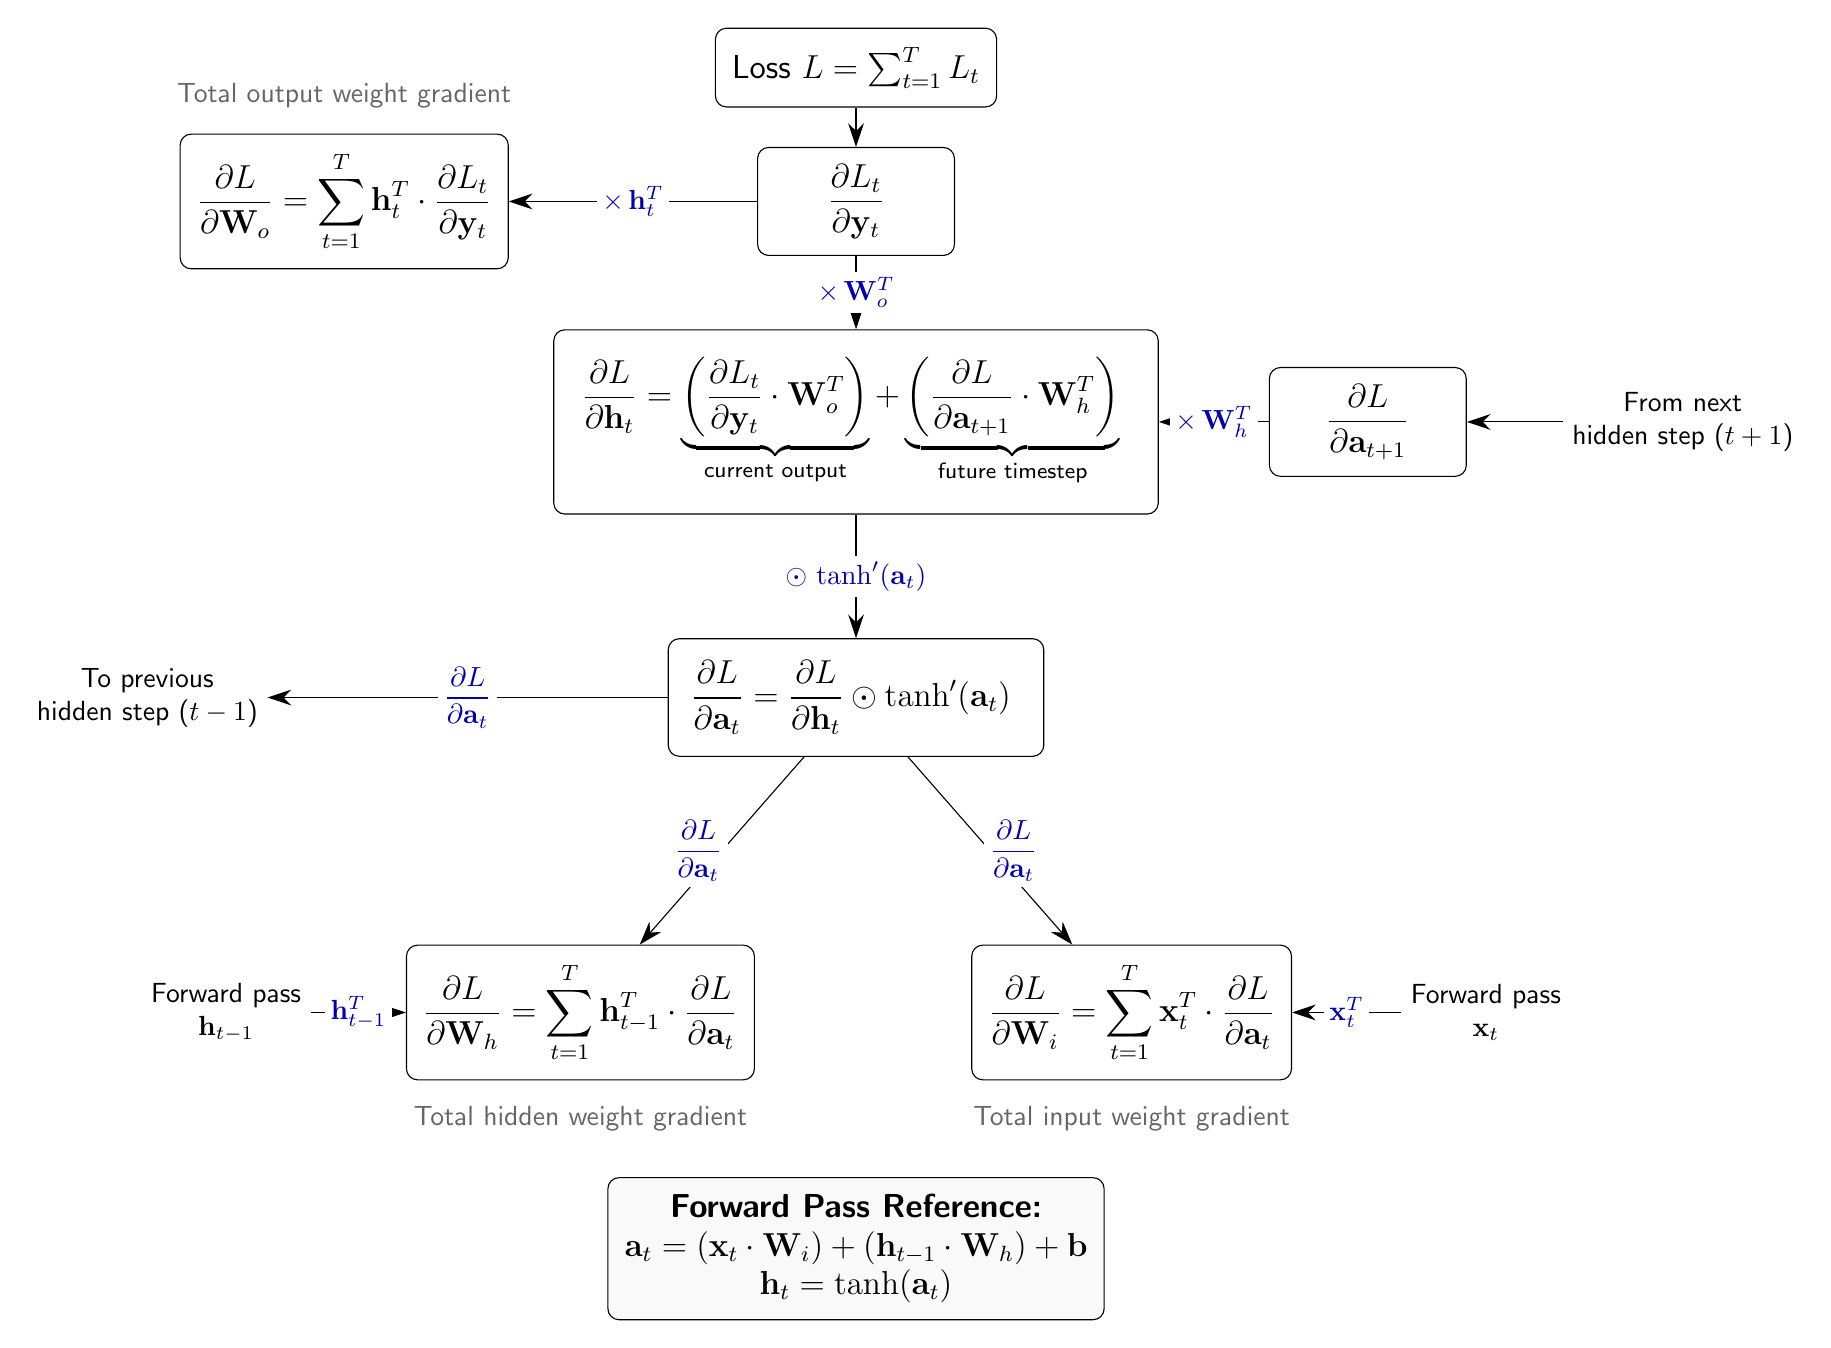
\begin{tikzpicture}[
    >={Stealth[length=3mm, width=2mm]},
    box/.style={draw, rounded corners, minimum width=2.5cm, minimum height=1cm, align=center, fill=white, font=\large, inner sep=6pt},
    txt/.style={align=center, font=\normalsize},
    edge_label/.style={fill=white, font=\normalsize, text=blue!70!black, inner sep=2pt}
]

% ================= Nodes =================

% Top level: Loss and Output Gradient
\node[box] (loss) at (0, 6.5) {Loss $L = \sum_{t=1}^{T} L_t$};
\node[box] (dy) at (0, 4.8) {$\displaystyle \frac{\partial L_t}{\partial \mathbf{y}_t}$};

% Mid-level: Output gradients (Summed over time)
\node[box] (dwo) at (-6.5, 4.8) {$\displaystyle \frac{\partial L}{\partial \mathbf{W}_o} = \sum_{t=1}^{T} \mathbf{h}_{t}^T \cdot \frac{\partial L_t}{\partial \mathbf{y}_{t}}$};

% Central level: The explicit hidden state gradient node with BPTT intuition
\node[box, inner sep=10pt] (dh) at (0, 2) {
    $\displaystyle \frac{\partial L}{\partial \mathbf{h}_t} = \underbrace{\left( \frac{\partial L_t}{\partial \mathbf{y}_t} \cdot \mathbf{W}_o^T \right)}_{\text{current output}} + \underbrace{\left( \frac{\partial L}{\partial \mathbf{a}_{t+1}} \cdot \mathbf{W}_h^T \right)}_{\text{future timestep}}$
};

% Lower Central: The activation derivative node
\node[box, inner sep=8pt] (da) at (0, -1.5) {
    $\displaystyle \frac{\partial L}{\partial \mathbf{a}_t} = \frac{\partial L}{\partial \mathbf{h}_t} \odot \tanh'(\mathbf{a}_t)$
};

% Horizontal temporal flow (Right side: from future)
\node[box] (from_next) at (6.5, 2) {$\displaystyle \frac{\partial L}{\partial \mathbf{a}_{t+1}}$};
\node[txt] (next_step_txt) at (10.5, 2) {From next \\ hidden step ($t+1$)};

% Horizontal temporal flow (Left side: to past)
\node[txt] (prev_step_txt) at (-9, -1.5) {To previous \\ hidden step ($t-1$)};

% Bottom level: Hidden and Input weight gradients (Summed over time)
\node[box] (dwh) at (-3.5, -5.5) {$\displaystyle \frac{\partial L}{\partial \mathbf{W}_h} = \sum_{t=1}^{T} \mathbf{h}_{t-1}^T \cdot \frac{\partial L}{\partial \mathbf{a}_{t}}$};
\node[box] (dwi) at (3.5, -5.5) {$\displaystyle \frac{\partial L}{\partial \mathbf{W}_i} = \sum_{t=1}^{T} \mathbf{x}_{t}^T \cdot \frac{\partial L}{\partial \mathbf{a}_{t}}$};

% Forward pass inputs for reference
\node[txt] (ht_prev) at (-8, -5.5) {Forward pass \\ $\mathbf{h}_{t-1}$};
\node[txt] (xt) at (8, -5.5) {Forward pass \\ $\mathbf{x}_t$};

% ================= Labels =================

\node[above=0.2cm of dwo, text=gray!80!black, font=\normalsize] {Total output weight gradient};
\node[below=0.2cm of dwh, text=gray!80!black, font=\normalsize] {Total hidden weight gradient};
\node[below=0.2cm of dwi, text=gray!80!black, font=\normalsize] {Total input weight gradient};

% ================= Edges =================

% Top level connections
\draw[->] (loss) -- (dy);
\draw[->] (dy) -- (dwo) node[midway, edge_label] {$\times \, \mathbf{h}_t^T$};

% Connecting gradients to the hidden node (operations explicitly on edges)
\draw[->] (dy) -- (dh) node[midway, edge_label] {$\times \, \mathbf{W}_o^T$};
\draw[->] (from_next) -- (dh) node[midway, edge_label] {$\times \, \mathbf{W}_h^T$};

% Connecting temporal nodes
\draw[<-] (from_next) -- (next_step_txt);

% Connecting hidden state to pre-activation
\draw[->] (dh) -- (da) node[midway, edge_label] {$\odot \, \tanh'(\mathbf{a}_t)$};

% Temporal connections directly to the past (removed redundant node)
\draw[->] (da) -- (prev_step_txt) node[midway, edge_label] {$\displaystyle \frac{\partial L}{\partial \mathbf{a}_t}$};

% Branching out to weight gradients (t contribution adding to the sum)
\draw[->] (da) -- (dwh) node[midway, edge_label, xshift=-0.3cm] {$\displaystyle \frac{\partial L}{\partial \mathbf{a}_t}$};
\draw[->] (da) -- (dwi) node[midway, edge_label, xshift=0.3cm] {$\displaystyle \frac{\partial L}{\partial \mathbf{a}_t}$};

% Forward pass inputs to weight gradients
\draw[->] (ht_prev) -- (dwh) node[midway, edge_label] {$\mathbf{h}_{t-1}^T$};
\draw[->] (xt) -- (dwi) node[midway, edge_label] {$\mathbf{x}_t^T$};

% ================= Forward Pass Definitions =================

\node[box, inner sep=6pt, fill=gray!5] (equations) at (0, -8.5) {
    \textbf{Forward Pass Reference:} \\
    $\mathbf{a}_t = (\mathbf{x}_t \cdot \mathbf{W}_i) + (\mathbf{h}_{t-1} \cdot \mathbf{W}_h) + \mathbf{b}$ \\
    $\mathbf{h}_t = \tanh(\mathbf{a}_t)$
};

\end{tikzpicture}
\end{document}